\section{Geometry Generation}

Designing a good model geometry is critical as it can save significant computational resources.
When designing a geometry the FEM user should try to represent the model geometry as accurately as possible while:
\begin{enumerate}
  \item Avoid unnecessarily fine details; these may require an excessively fine mesh to resolve.
  \item Leverage symmetry to reduce the domain size over which solution must be effected, and thereby the mesh can be made finer in a smaller portion of the domain.
\end{enumerate}\par
Achieving these goals is not always straightforward, and success depends on the skill of the modeler and on the available tools.
Typically a model geometry is constructed in some computer assisted design (CAD) software, and the particular tools available in these packages vary.
While not absolutely necessary, the usa of a CAD package outside of the COMSOL solver might sometimes make development of the domain description easier.\par

\begin{figure}[htb!]
  \centering
  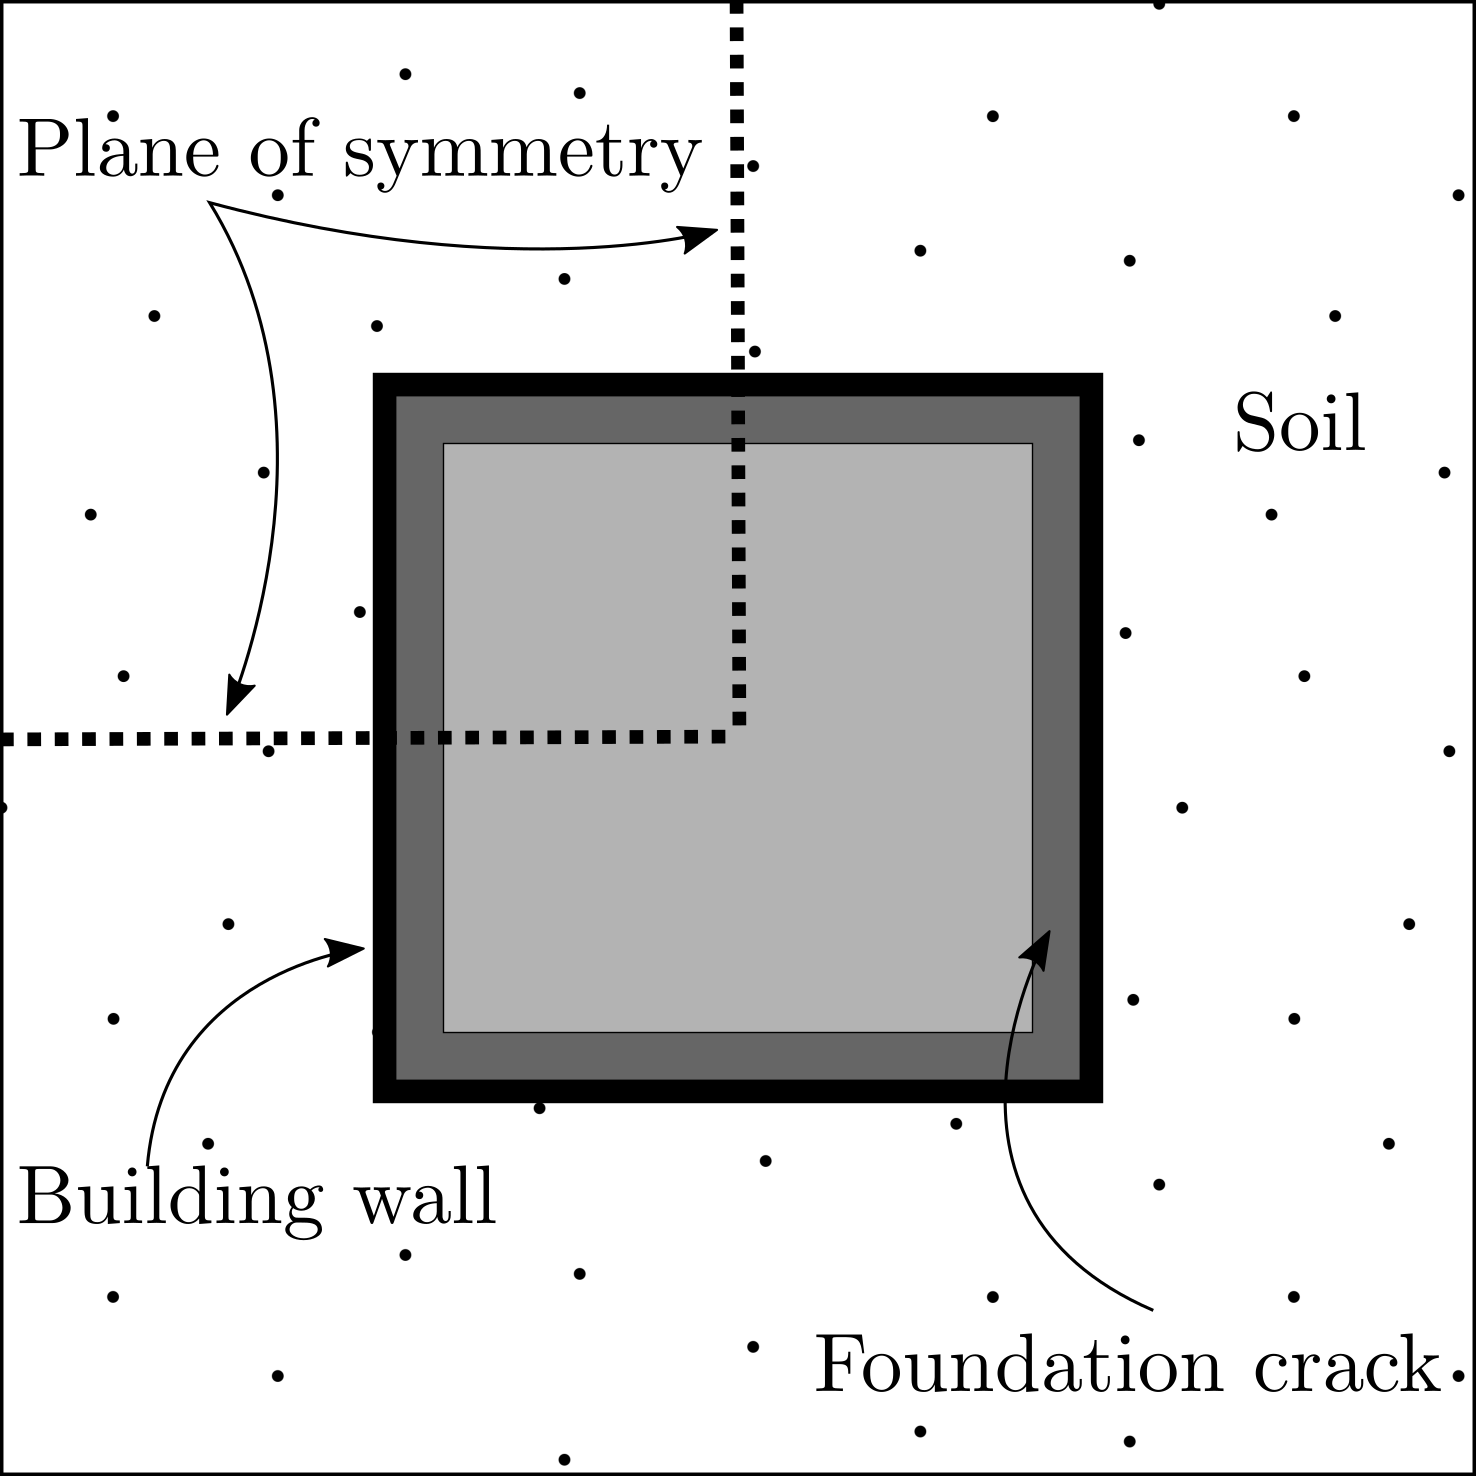
\includegraphics[width=0.75\textwidth]{symmetry.png}
  \caption{Birds-eye view of the VI scenario, showing the foundation and the breach, building wall, as well as the plane of symmetry that allows only a quarter of the total domain to be generated.}
  \label{fig:symmetry}
\end{figure}

COMSOL has a built-in geometry generation tool, which allows the construction of advanced geometries by performing various operations on simpler geometries, e.g. a cylinder and half sphere can be combined to make a rivet.
But as noted, it is also possible to import pre-generated geometries from other CAD software.
For present illustrative purposes, we will create our own geometry.\par

The interior of the house itself will not be explicitly modeled, instead we only consider the soil surrounding the house.
This is done for the simple reason that it is not important to model the interior of the house.
Once the contaminant is in the structure, the damage, so to speak, has been done.
We are interested in how fast the contaminant enters from the soil, which is what determines indoor contaminant concentration.
In addition, typical building interiors are simply too heterogenous to generalize in any meaningful way.
Trying to explicitly model the interior so as to offer insights into indoor concentration variations while at the same time modeling the necessary subsurface transport, would be prohibitively expensive.
Instead the interior is implicitly modeled as a CSTR and simply coupled with the explicit soil and foundation geometry via the foundation crack boundary.\par

One of the nice properties of the described VI scenario is that, due to symmetry, we only need to explicitly model a quarter of it (see Figure \ref{fig:symmetry}).
This reduces the number of required mesh points by 75\%, which is a huge computational saving.
To create the specified geometry, see the instructions for geometry generation in the appendix.

\begin{figure}[htb!]
  \centering
  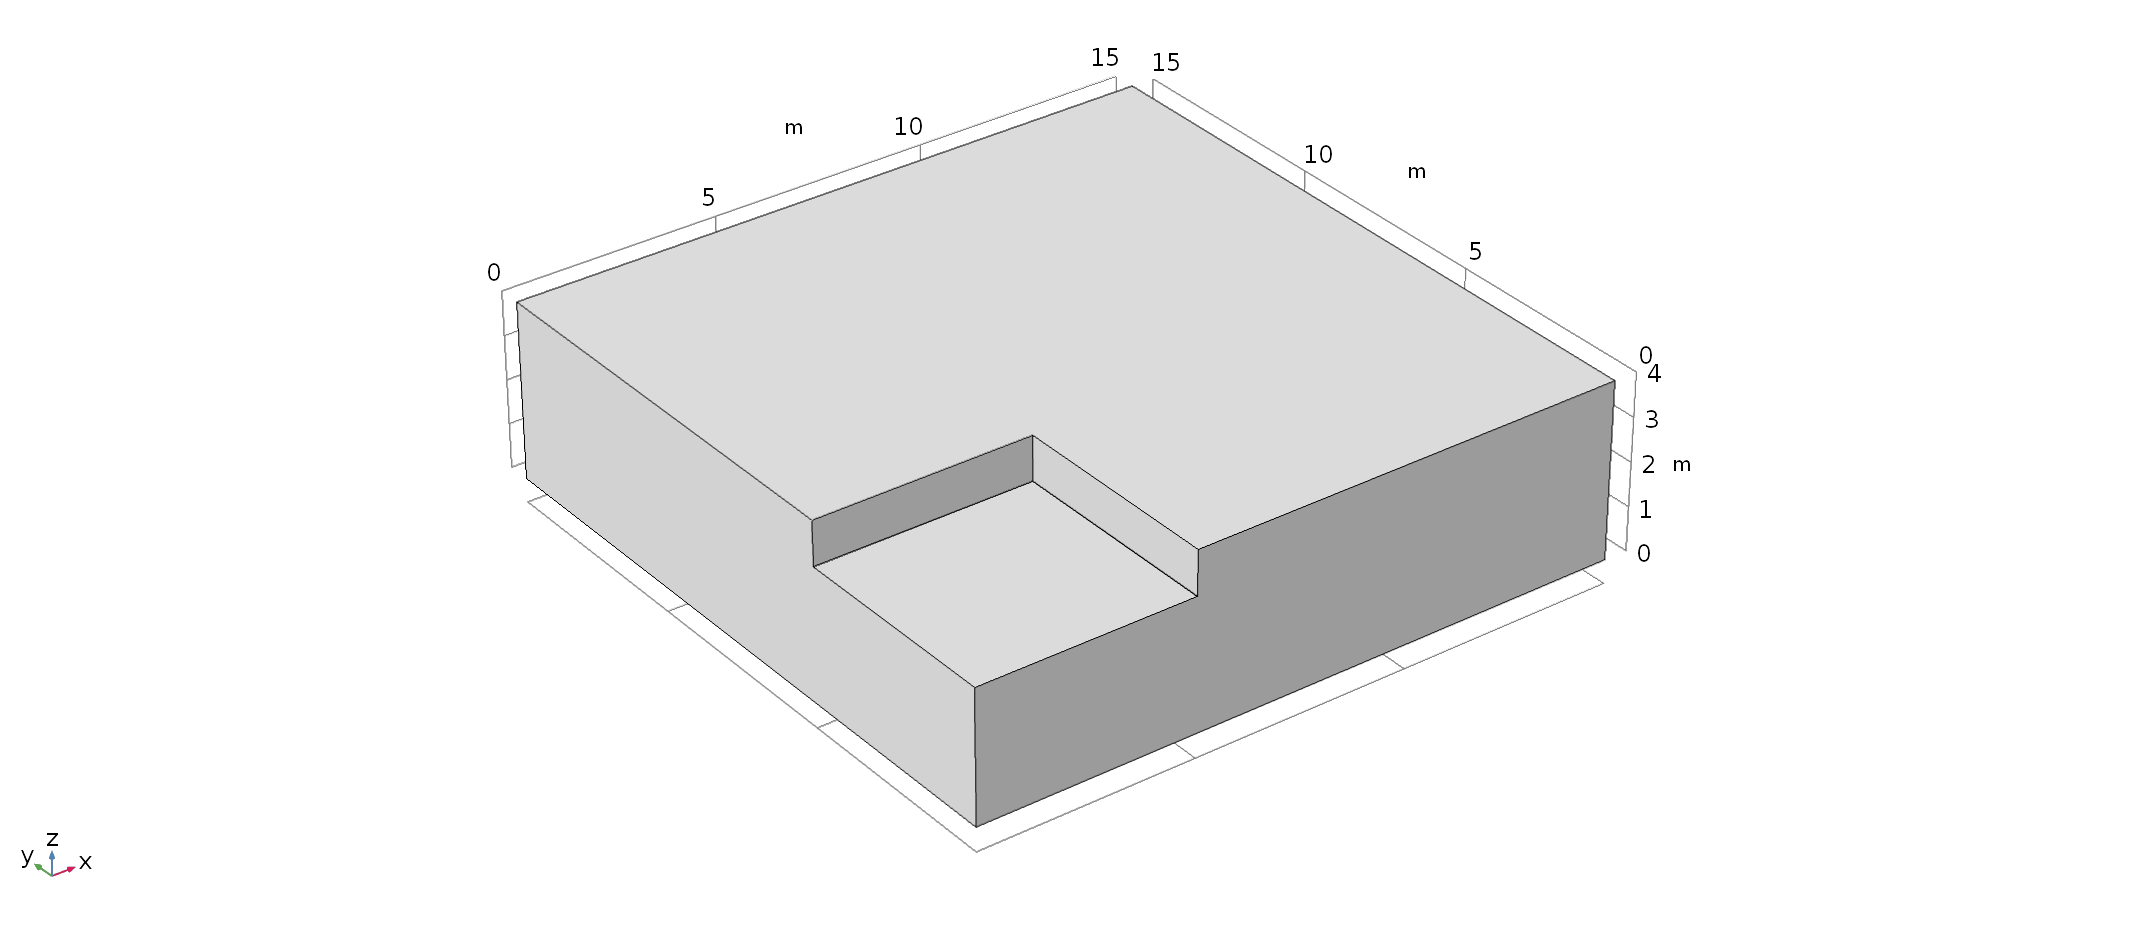
\includegraphics[width=\textwidth]{vi_model.png}
  \caption[VI model geometry in COMSOL]{The complete geometry of the VI scenario as implemented in COMSOL.}
  \label{fig:geometry}
\end{figure}
